>\section{Description of the task}\label{sec:task_description}
This section serves as a preliminary one for the rest of the report. The main task
of interest is briefly recalled and several frames of reference are introduced within
the typical setup in which the task is performed. These frames of reference, along
with some notations and conventions, will be useful to easily identify the quantities
that belong to the state of the controllers developed in the next sections of this report.

\subsection{Typical set-up}
The typical setup, as shown in figure \ref{fig:frames}, consists of a $7$-joints KUKA LWR $4$+
anthropomorphic manipulator equipped with an hand-like end-effector, a table and an object that the hand is not
able to grasp using its primitives.
\begin{figure}[h]
  \centering
  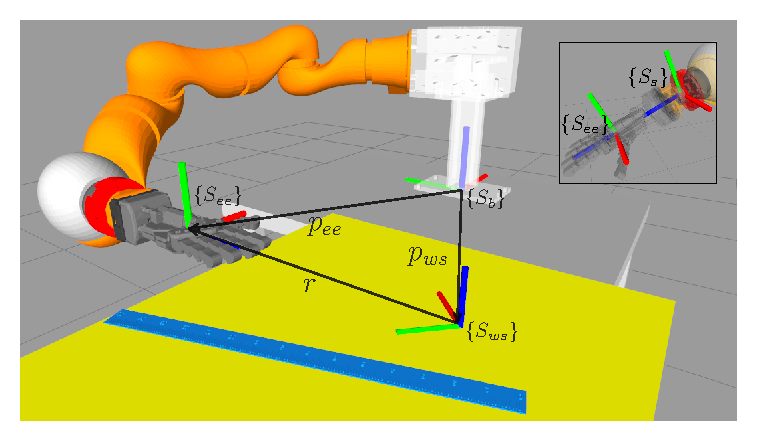
\includegraphics[scale=1.1]{frames_new.pdf}
  \caption{Typical set-up with reference frames \label{fig:frames}}
\end{figure}
Then the task to be performed consists in dragging the object on the table, hence exploiting
the environmental constraints offered by the surface of the table, until the object sticks
out of the border of the table and a standard grasp is feasible. Also the dragging phase should
be accomplished without damaging the object or the hand because of too high contact forces between
the object and the surface of the table or between the object and the hand.
For this reason the manipulator is equipped with a force/torque sensor (fig. \ref{fig:sensor}) which is rigidely attached
to the last link of the robot and measures forces and torques exchanged at the wrist of the robot.
The hand is connected to the sensor using a mounting plate and a clamp.
\begin{figure}[h]
  \centering
  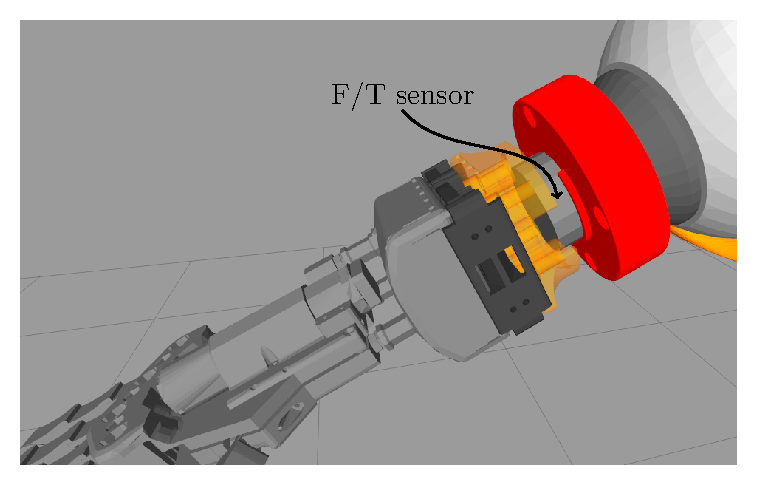
\includegraphics[scale=1]{sensor.pdf}
  \caption{Set-up of the force/torque sensor.\label{fig:sensor}}
\end{figure}

\subsection{Division of the task in phases}\label{sec:task_division}
The dragging phase described above can be considered as the \emph{final} part of a more
complex task which should be divided, at least, in three parts:
\begin{itemize}
\item[-] approaching phase in which the robot moves the hand near the object of interest;
\item[-] contact phase in which the contact between the hand and the object takes place;
\item[-] dragging phase.
\end{itemize}

In the rest of the this report more attention is given to the dragging phase since it is the phase
where the hybrid force position strategy is used. As regards the contact phase the experimental results,
presented in the last section, show that it can be achieved using the same controller used in the dragging
phase. The approaching phase is also described in a separate section.

\subsection{Frames of reference}\label{sec:frames}
In order to develop a control system that is able to regulate the position of the object
and the force exerted on it, i.e. an hybrid force position control system, while the hand
is dragging the object on the table
a natural choice for a basis in which express the commanded positions and forces is that of
an inertial reference frame with the origin $W$ on a point of the table and the $x$ and $y$ axes parallel to the surface
of the table
\[
\{S_{ws}\} = \{W; x_{ws}, y_{ws}, z_{ws} \}
\]
where \emph{ws} stands for ``workspace'' since the table represents the intended workspace
for the robot. This choice allows to specify the commanded position as 2-dimensional vector
with components along the directions $\hat{\vec{i}}_{ws}$ and $\hat{\vec{j}}_{ws}$ and the
commanded force as a positive scalar along the direction $-\hat{\vec{k}}_{ws}$.
A quantity related to this reference frame is the vector $\vec{r}$ going from the origin $W$
to the center of the palm of the hand.
\par
A second reference frame to be introduced is an inertial frame fixed to the main base of the robot
\[
\{S_b\} = \{B; x_b, y_b, z_b \}
\]
Similarly to $\vec{r}$ the vector $\vec{p}_{ee}$ goes from $B$ to the center of the palm of the hand.
It should be noted that frames $\{S_{ws}\}$ and $\{S_b\}$ have no relative orientation and that
the vector $\vec{p}_{ws}$ going from $B$ to $W$ is constant. As a consequence the vector $\vec{r}(t)$
can be express as
\[
\vec{r}(t) = \vec{p}_{ee}(t) - \vec{p}_{ws}
\]
where $\vec{p}_{ws}$ is known and $\vec{p}_{ee}(t)$ is given by forward kinematics
numerical routines such as those offered by the library KDL used in this project.
The frame $\{S_b\}$ is also the frame in which the library KDL expresses quantities
like the vector $\vec{p}_{ee}$, the Jacobians and their derivatives.
\par
Other reference of frames of interest are those fixed to the end-effector
\[
\begin{split}
  &\{S_{fl}\} = \{F; x_{fl}, y_{fl}, z_{fl} \}\\
  &\{S_{ee}\} = \{E; x_{ee}, y_{ee}, z_{ee} \}
\end{split}
\]
where $F$ corresponds to the center of the wrist of the robot and $E$ is in the center
of the palm of the hand. These frames, that have no relative orientation,  are of interest
mainly because the signal produced by the force/torque sensor are expressed in these frames.

\subsection{Notation and convention}
In the rest of this report the following notation will be used to express any quantity $X$ encountered:
\[
\prescript{b}{}{X}_p
\]
where $b$ specify the reference frame $\{S_b\}$ in which $X$ is expressed and, whenever
$X$ is a wrench or a Jacobian $J$ such that $X\vec{\dot{q}}$ is a twist, $p$ specify the
reference point of that wrench or that twist. In case $X$ is an analytical Jacobian or $X$ is a vector
containing \emph{also} angular displacement or angular rates it should be clear that the specification
of a basis has no meaning and it applies only to a part of the vector.
\par
This notation is very general and sometimes the prescript $b$ and/or the subscript $p$ will
be missing when they are clear from the context.

\newpage

